\section{Conclusions}

Here we present some conclusions drawn from our visualisations.

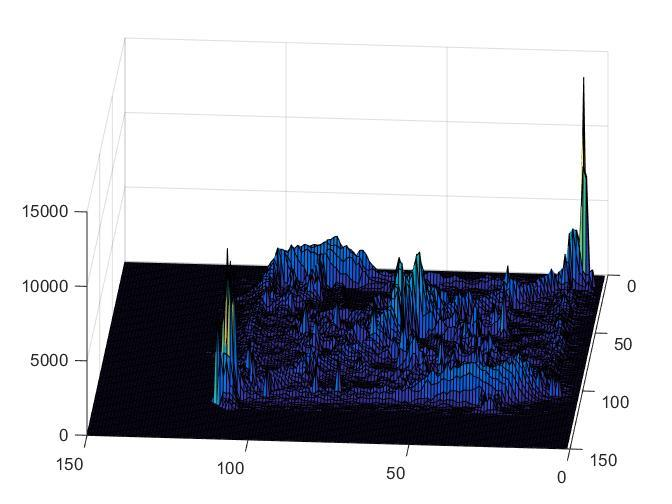
\includegraphics[width=\textwidth]{HM3D}
Here we show a raw, unnormalized 3D heatmap generated in MatLab. It shows two spikes on the starting areas. These might be the player starting positions, but almost look like outliners and might also indicate some errors.

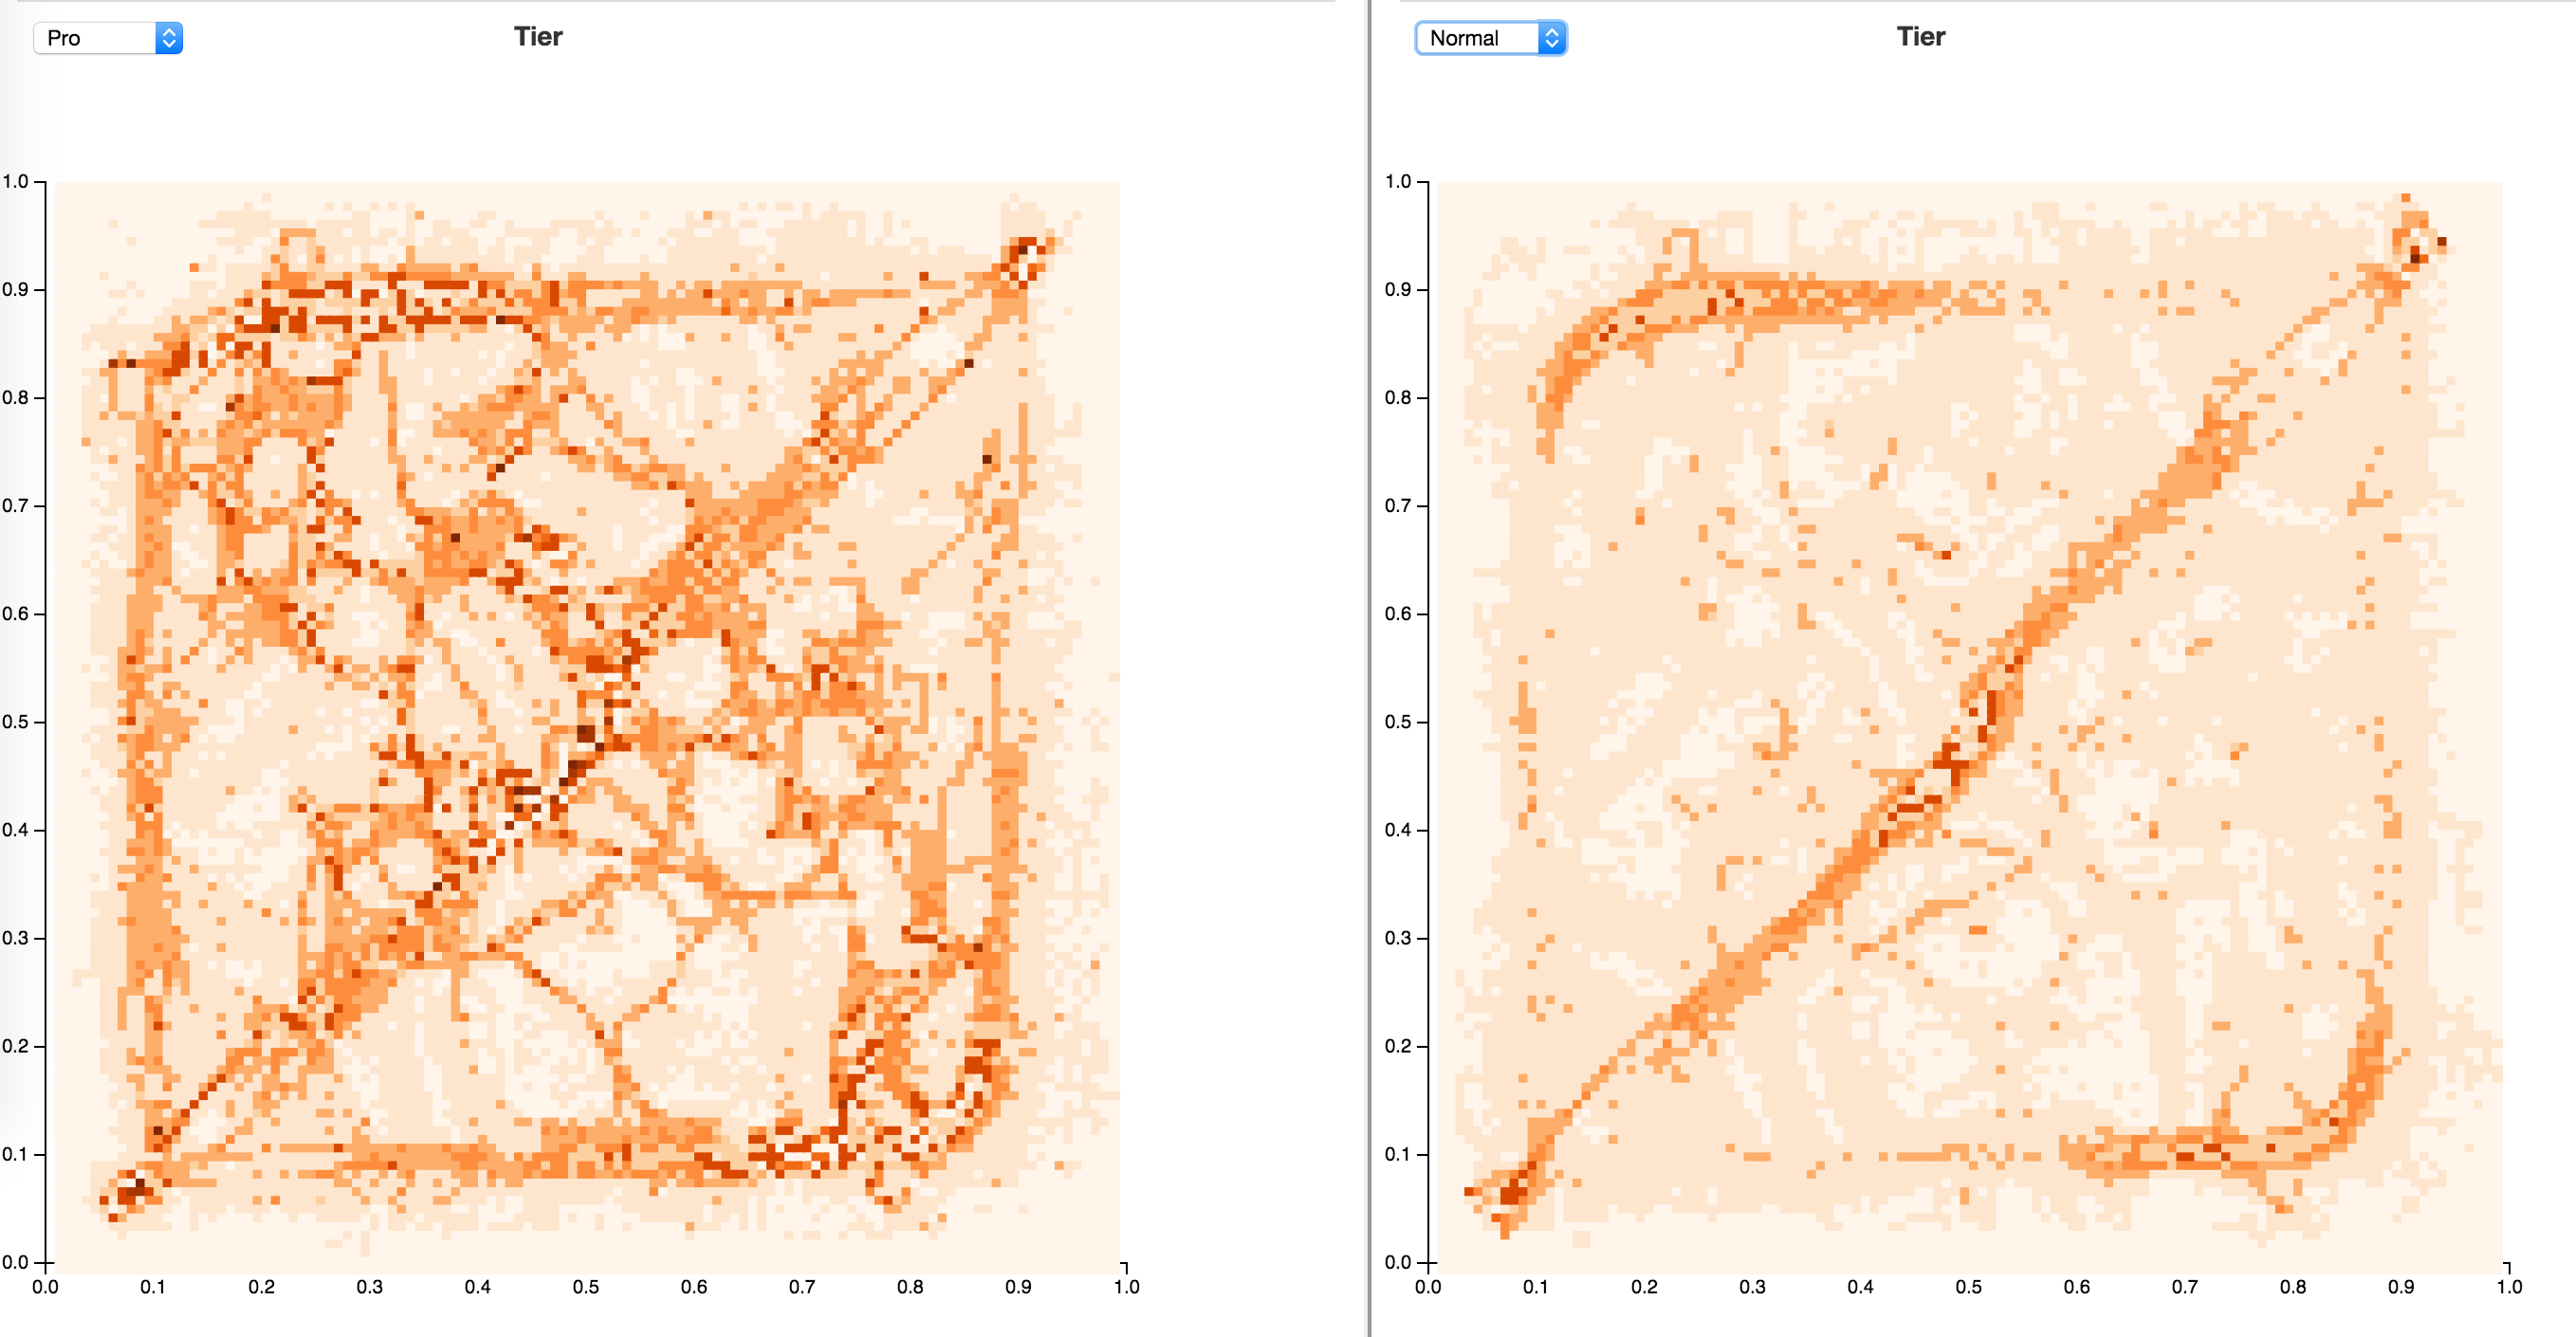
\includegraphics[width=\textwidth]{HM_tiers}

This image compares the heatmaps from low tier and pro tier. We can clearly see how the normal skill tier mostly fights in lanes and rarely fights in the jungle area, while the pro tier spends a lot more time in the jungle.

Here we see the early game, mid game and end game distributions from one match.

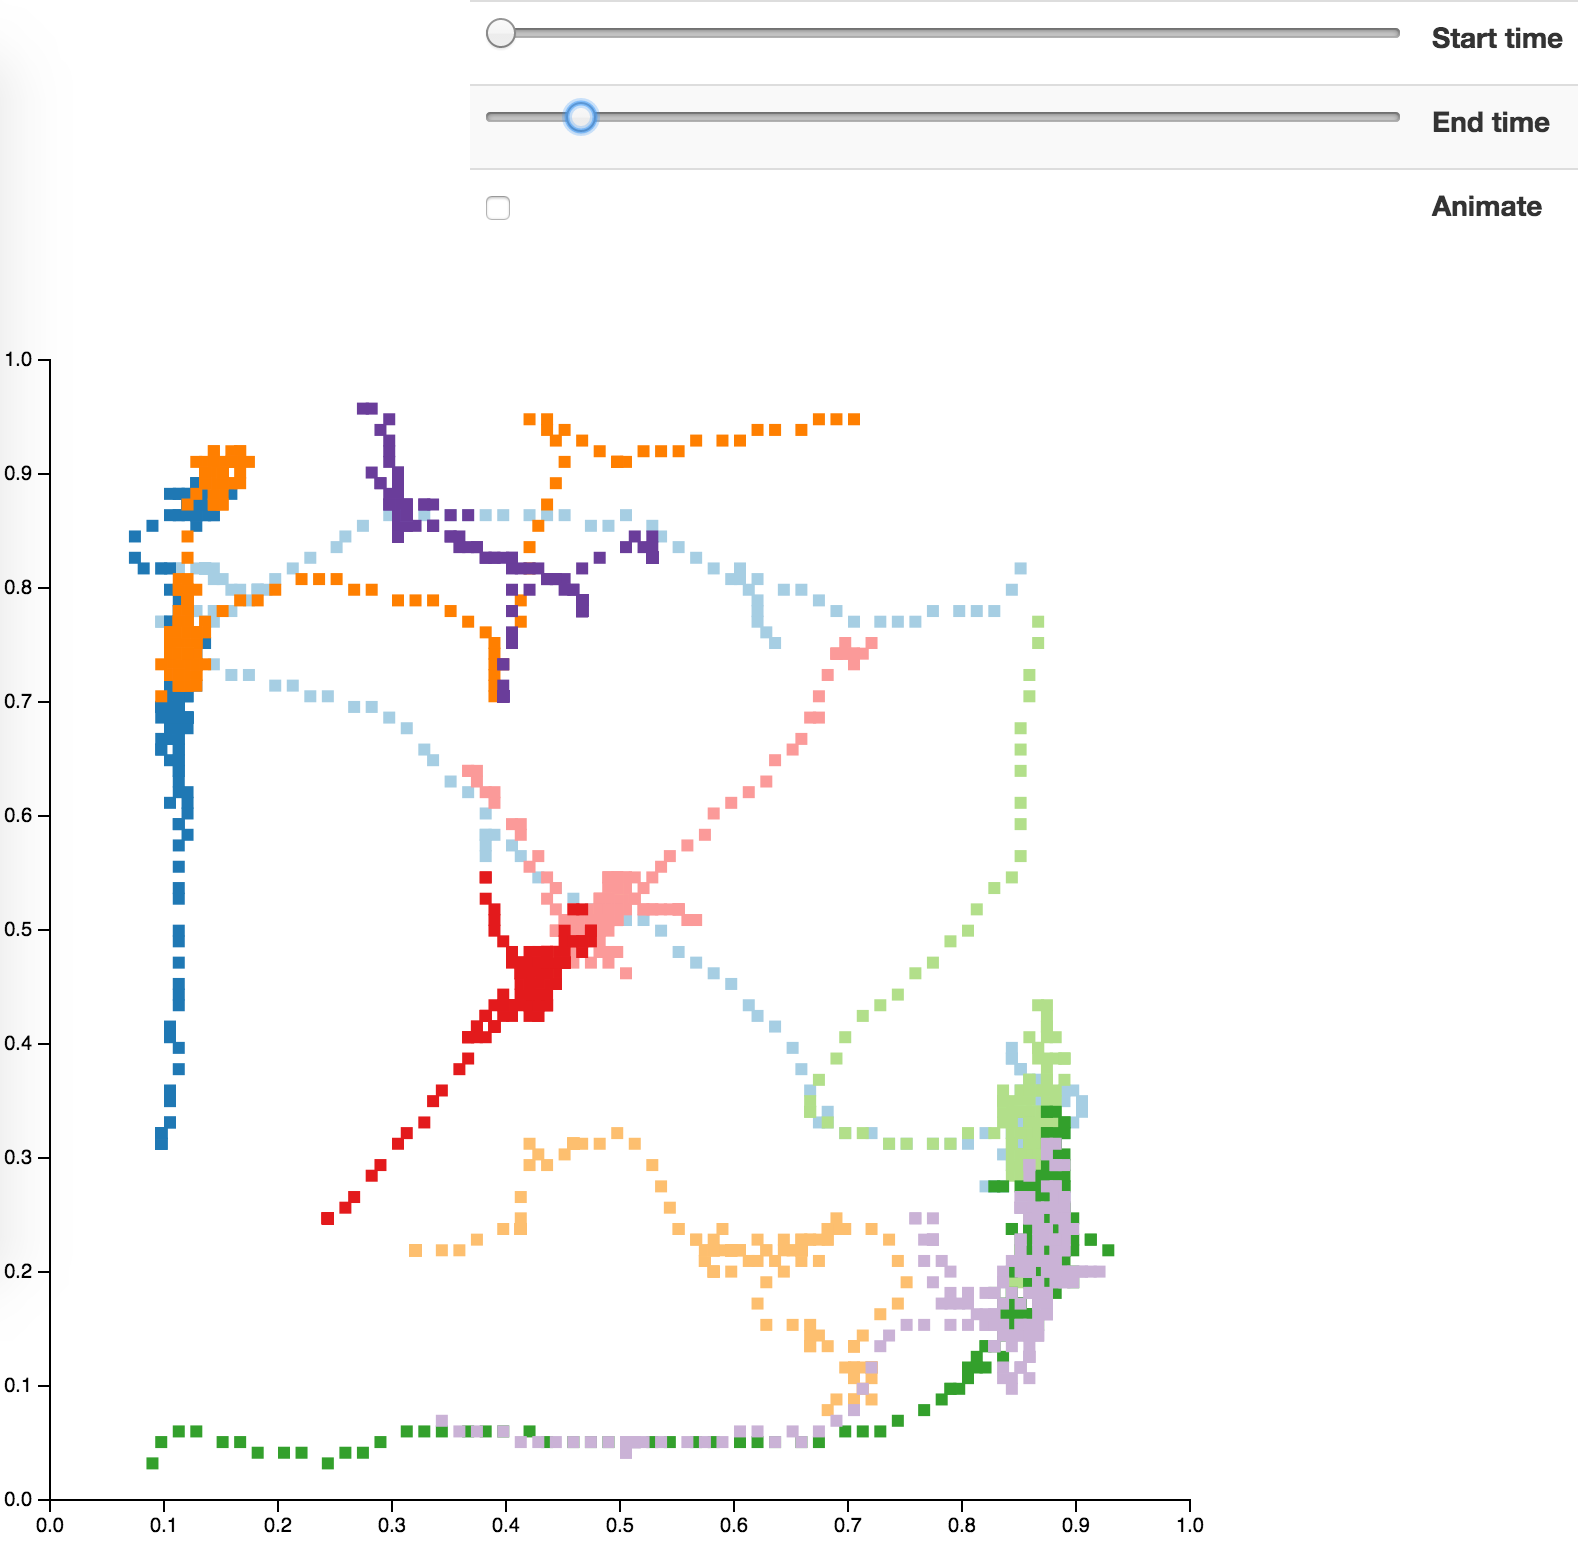
\includegraphics[width=0.7\textwidth]{earlygame}

In the early game we see the players moving into their respective lanes and exchange some blows.

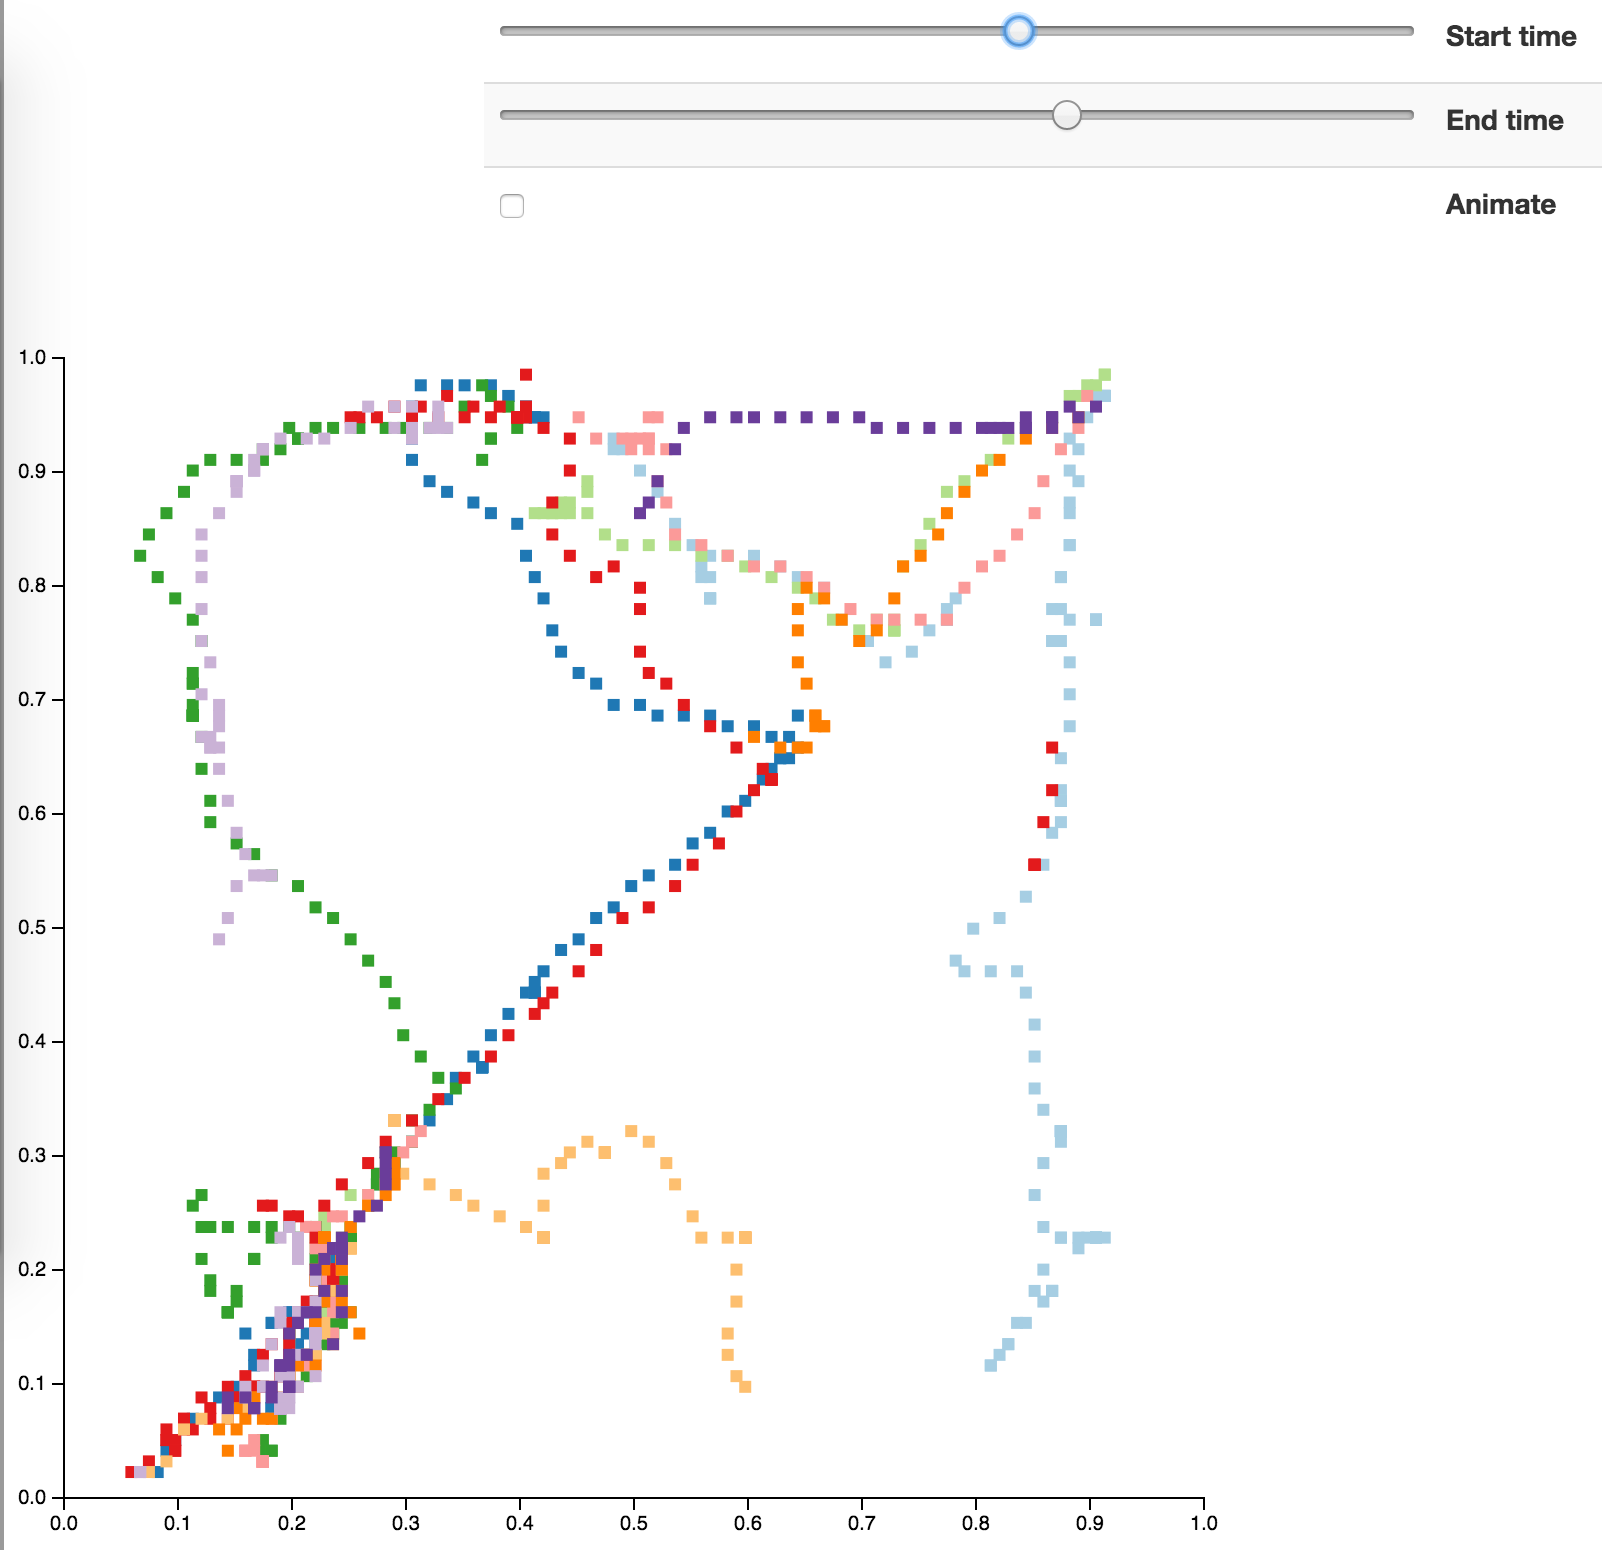
\includegraphics[width=0.7\textwidth]{midgame}

In the late-midgame we see that the game progressed out of their laning phases, and the action is moving towards the bottom team's base. We can see that they most probably lost the middle lane and are behind.

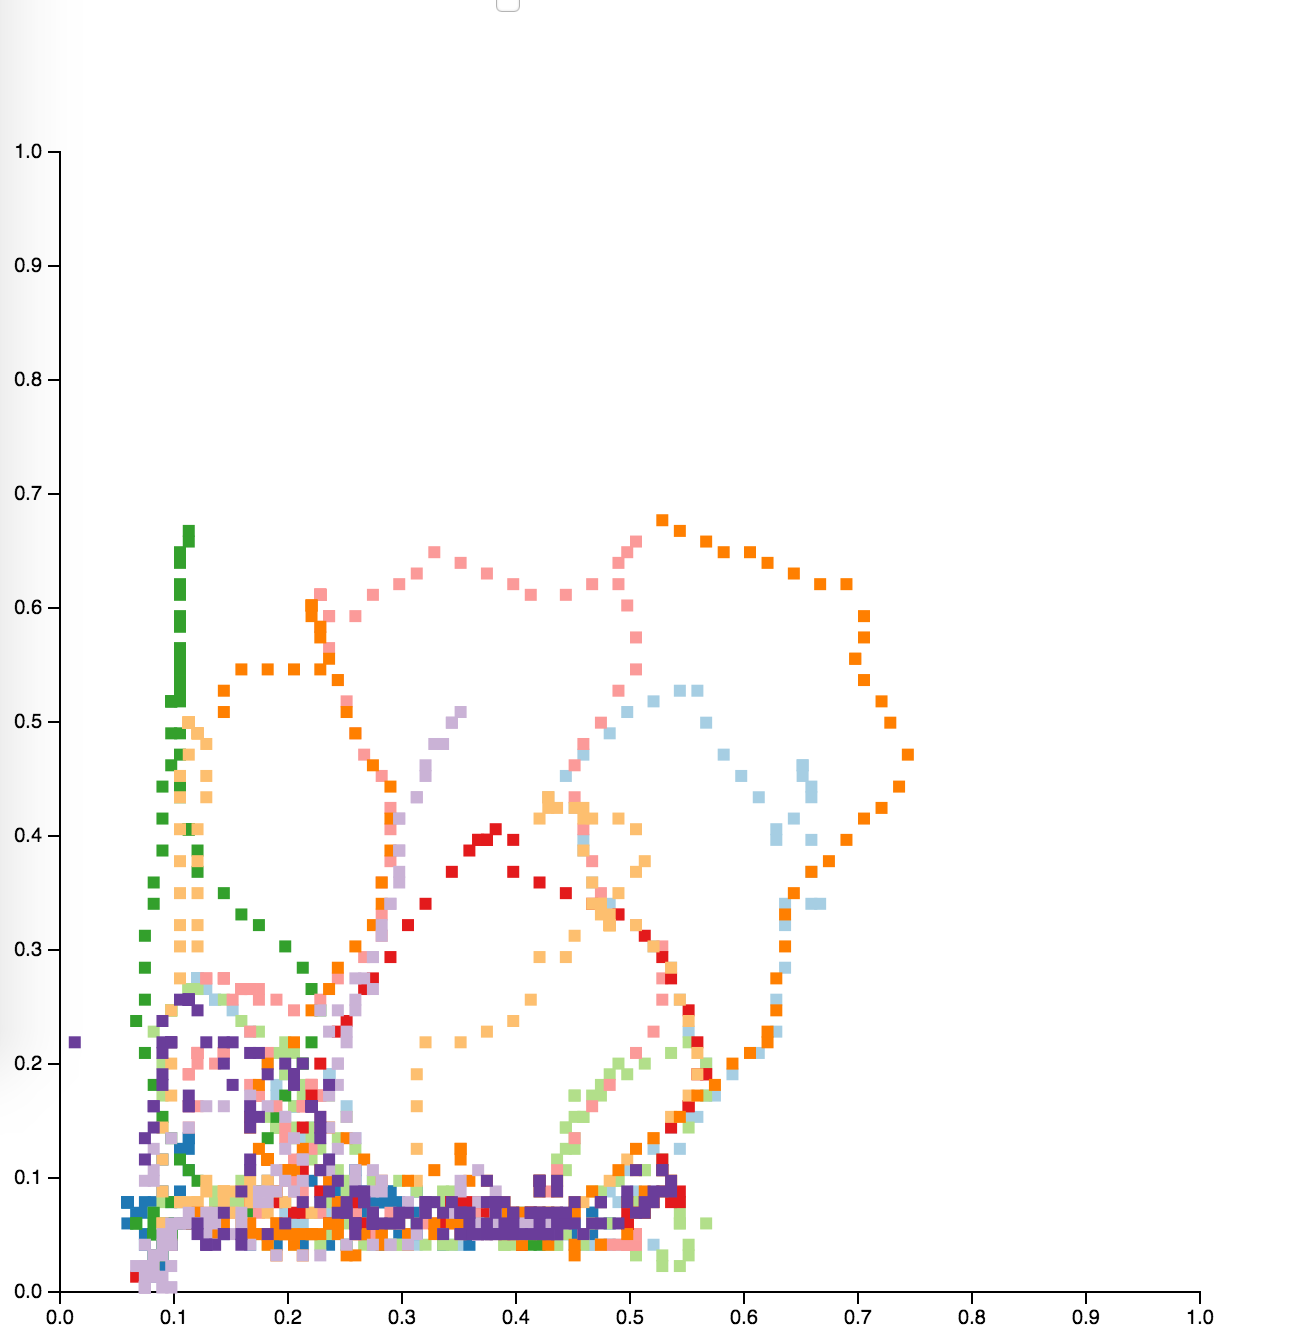
\includegraphics[width=0.7\textwidth]{lategame}

Late game confirms this by exclusively showing heavy fighting in the bottom lane and the bottom team's base. The game ended here, so we can conclude that the top team won.

